\documentclass{article}
\usepackage[utf8]{inputenc}
\usepackage[a4paper, total={6.5in, 9in}]{geometry}
\usepackage{fancyhdr}
\usepackage{amsmath, amsthm, amsfonts, mathrsfs}
\usepackage{xcolor}
\usepackage{mathtools, float, subfig}
\renewcommand{\labelenumii}{(\roman{enumii})}

\newcommand{\rr}{\mathscr{R}_0}

\setlength{\headsep}{4em}
\pagestyle{fancy}
\setlength{\parindent}{0cm}
\setlength{\parskip}{1em}

% ASSIGNMENT INFORMATION
\newcommand{\class}{MATH 490}
\newcommand{\hwnumber}{3}

\lhead{Braden Hoagland (bch29)}
\chead{{\class} - HW {\hwnumber}}
\rhead{\today}

\begin{document}

\section{SEIR Model}

Below are the projected values of $S(t), E(t), I(t)$, and $R(t)$ in the range $t \in [0, 500]$. The model paramters used are $\gamma = 0.1, \beta=0.24$, and $a=1/3$, and the initial condition is $(S_0, E_0, I_0, R_0) = (1-2*10^{-6}, 0, 2*10^{-6}, 0)$. The SIR model did not take into account $E_0$ or $a$.
\begin{figure}[H]
	\centering
	\subfloat[SIR Model through time]{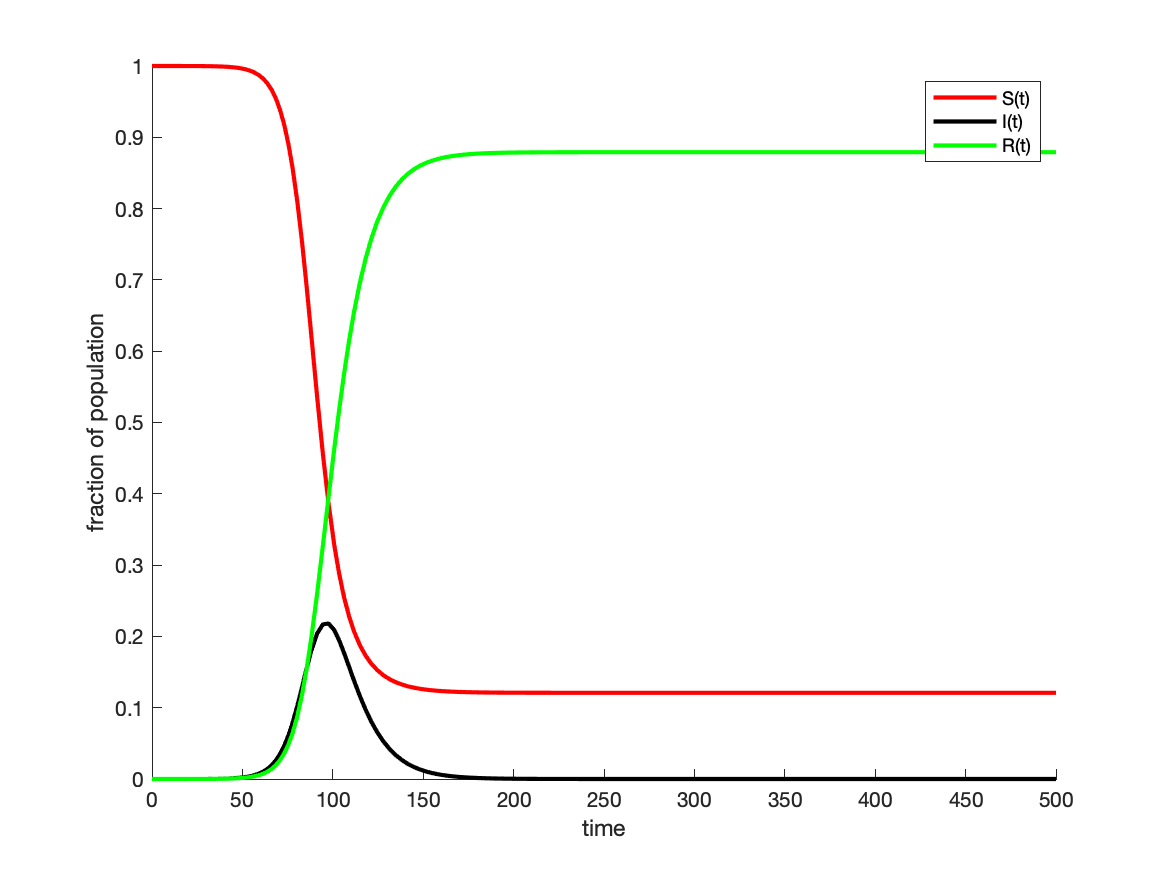
\includegraphics[scale=0.3]{img/time-SIR.png}}
	\subfloat[SIR Model in $SI$ space]{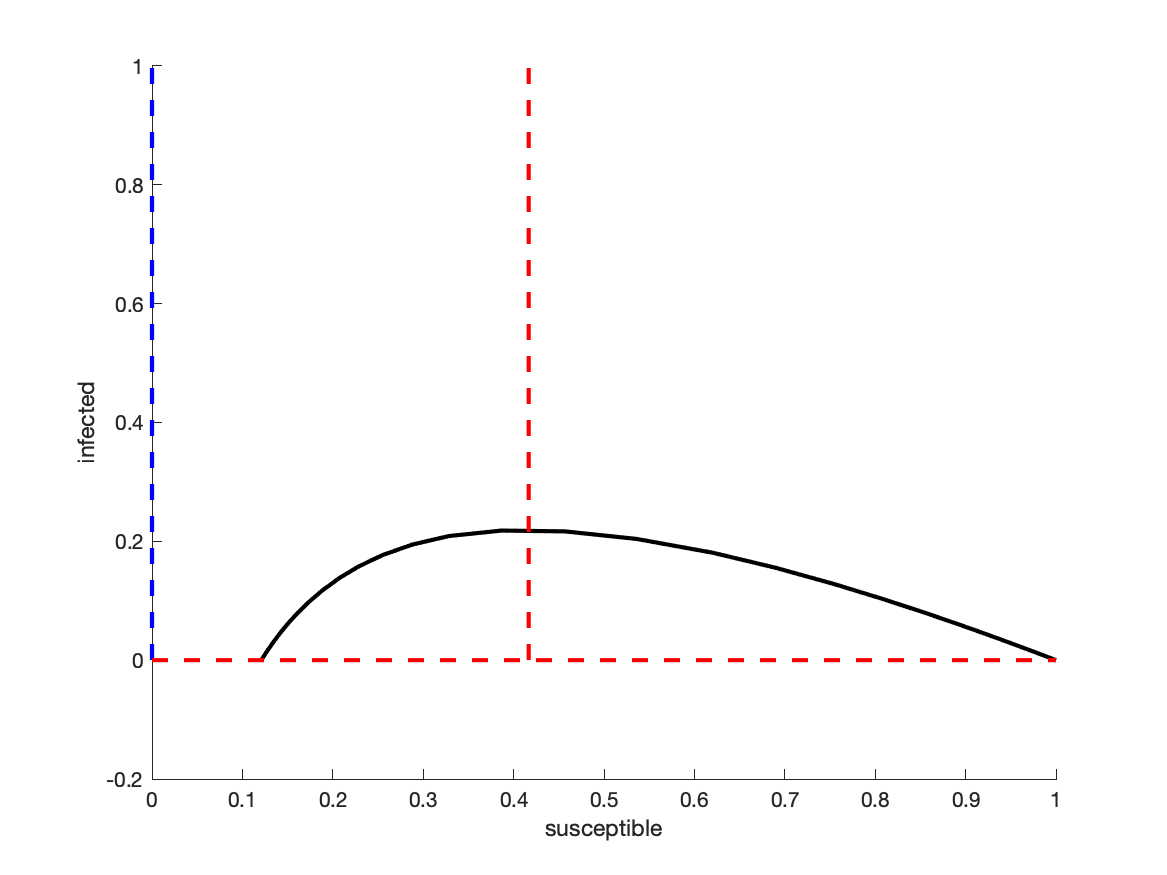
\includegraphics[scale=0.3]{img/SI-SIR.png}}
\end{figure}
\begin{figure}[H]
        \centering
        \subfloat[SEIR Model through time]{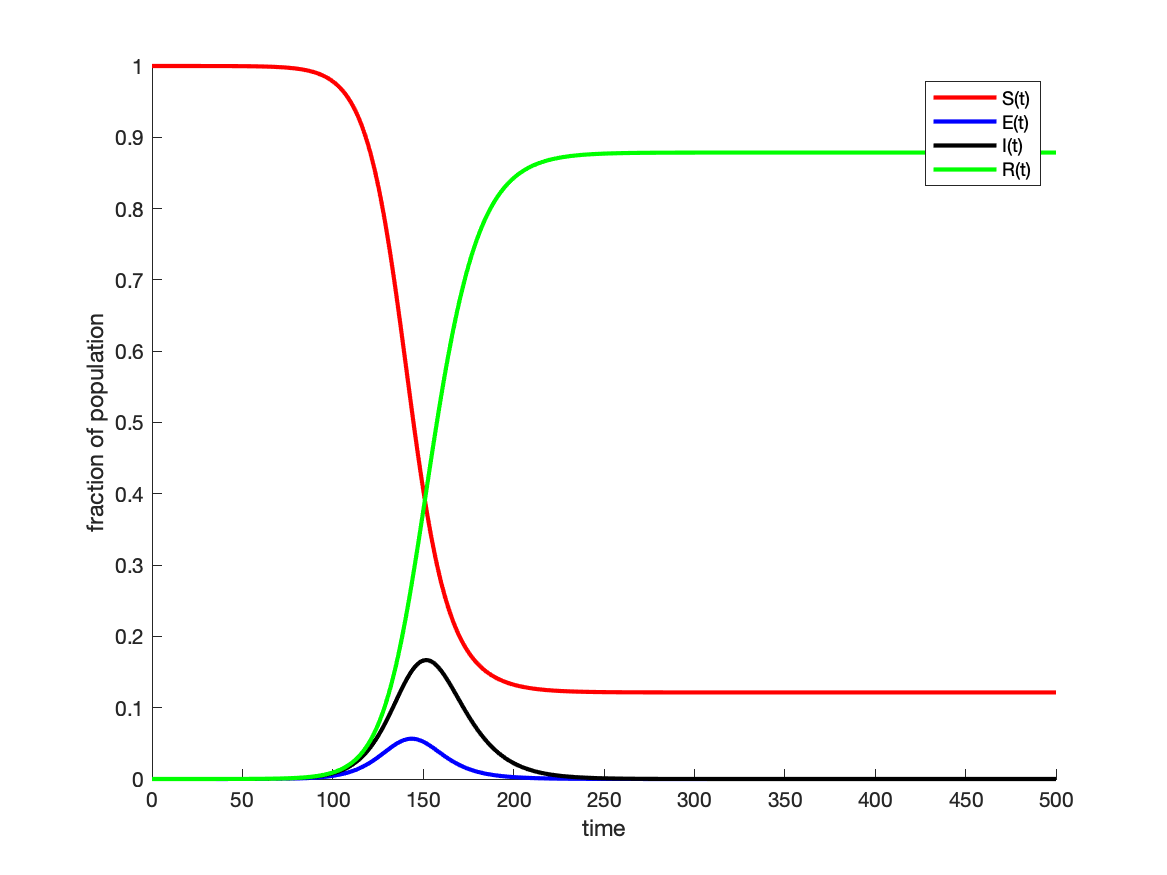
\includegraphics[scale=0.3]{img/time-SEIR-0.33.png}}
        \subfloat[SEIR Model in $SI$ space]{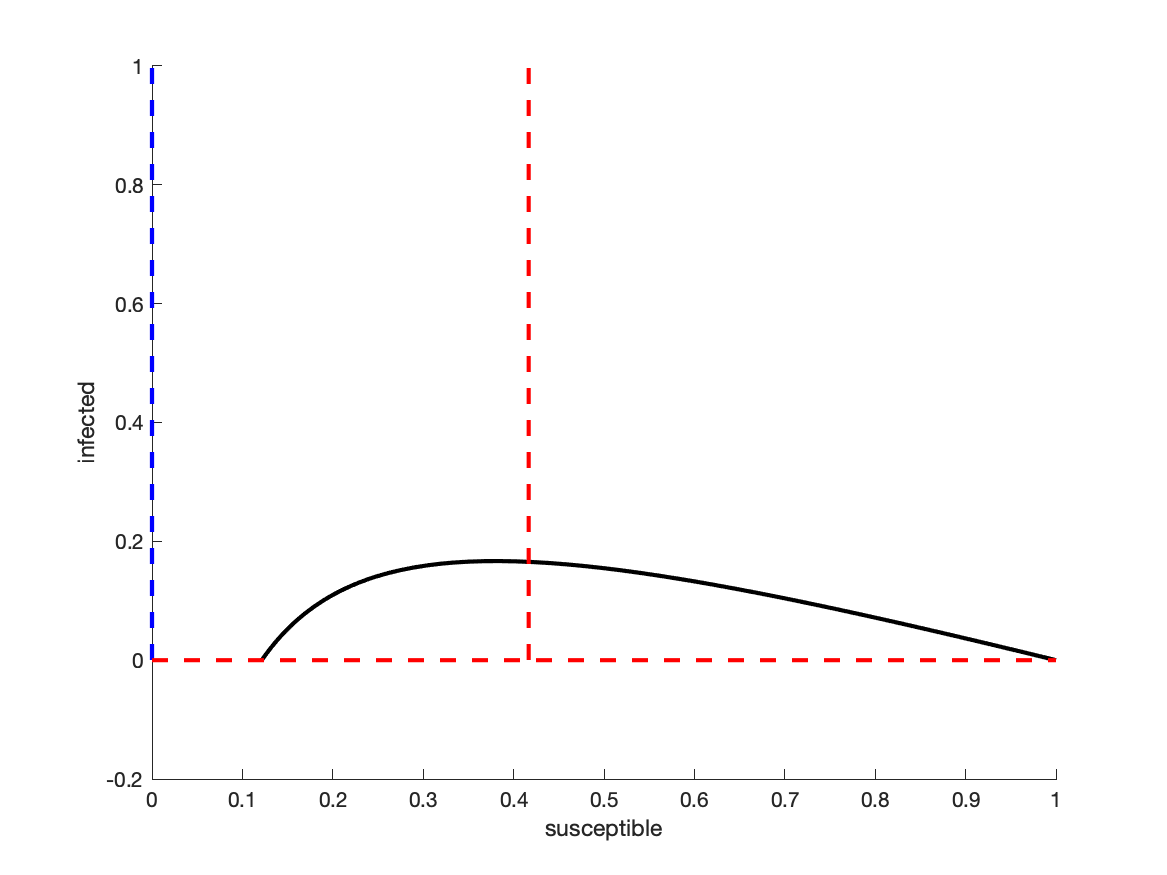
\includegraphics[scale=0.3]{img/SI-SEIR-0.33.png}}
\end{figure}
Qualitatively, these plots show that the SIR model has higher peak than the SEIR model, as well as overall lower values of $I(t)$ relative to $S(t)$ throughout the infection period. The desired statistics for each model are
\begin{center}
	\begin{tabular}{|c|c|c|}
		\hline
		& SIR & SEIR \\
		\hline
		Days until peak & 97.6 & 151.3 \\
		Height of peak & 0.22 & 0.17 \\
		Final epidemic size & 0.8791 & 0.8786 \\
		\hline
	\end{tabular}
\end{center}
where the final epidemic size was approximated by $1 - S(500)$. From this it can be seen that the SIR model predicted an earlier and sharper peak than the SEIR model, although the final proportion of people infected was essentially the same.

The same time curves are plotted below, but this time just with the results of the SEIR model and with $a$ parameter values of $1/9, 1/3$, and $0$.
\begin{figure}[H]
        \centering
        \subfloat[$a=1/9$]{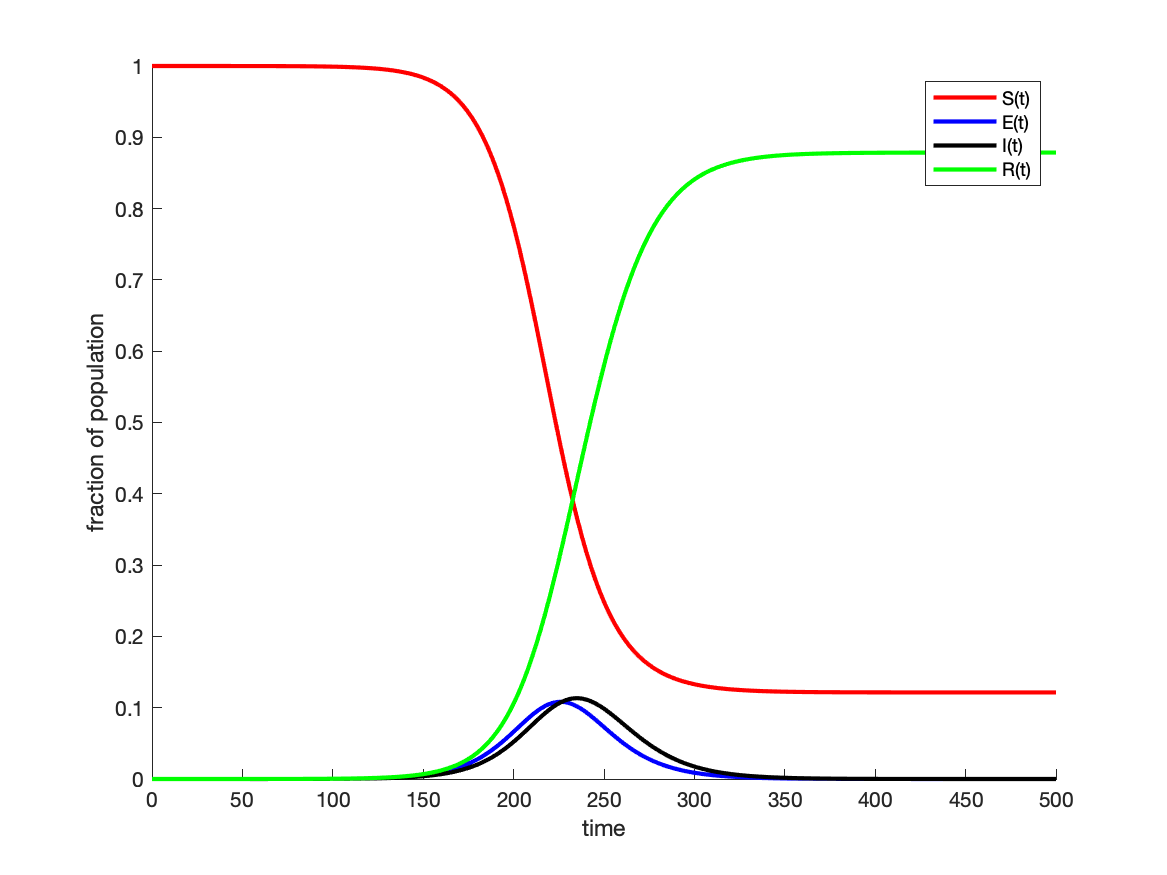
\includegraphics[scale=0.3]{img/time-SEIR-0.11.png}}
        \subfloat{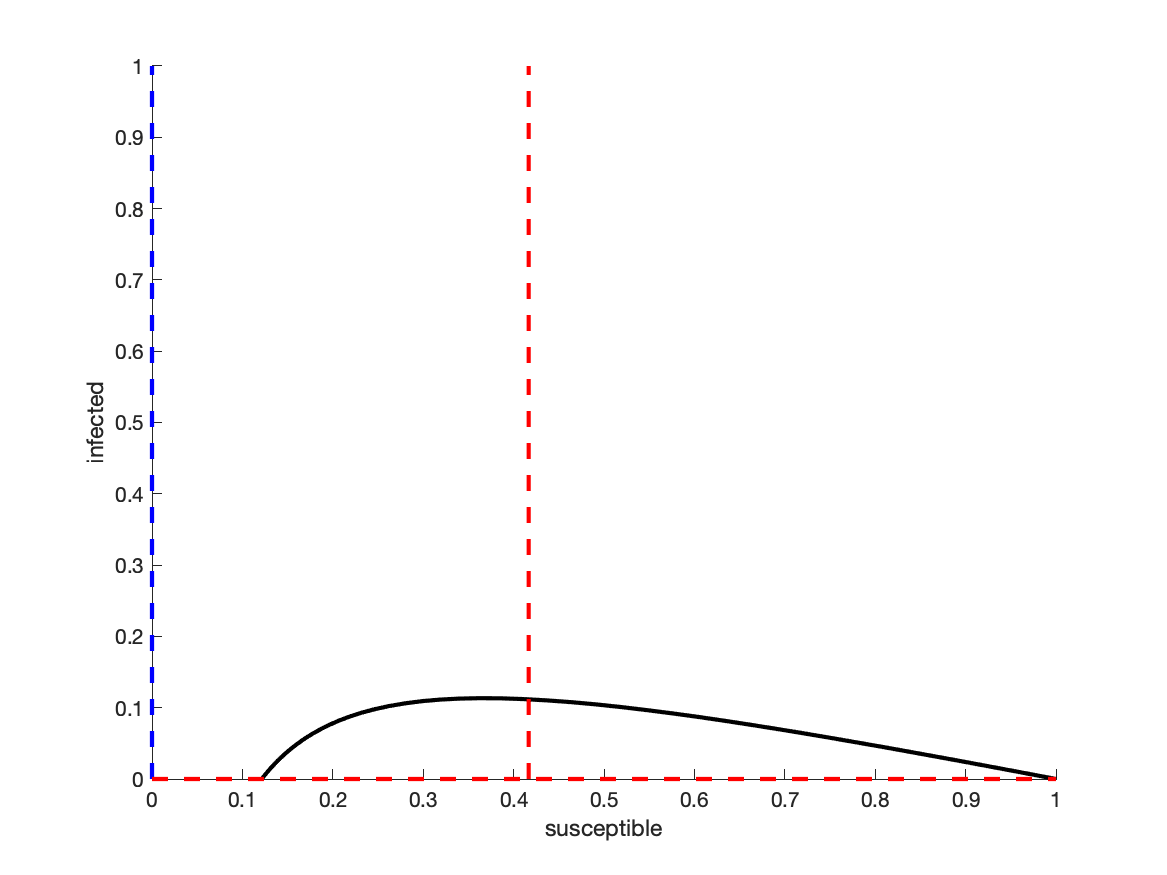
\includegraphics[scale=0.3]{img/SI-SEIR-0.11.png}}
\end{figure}
\begin{figure}[H]
        \centering
        \subfloat[$a=1/3$]{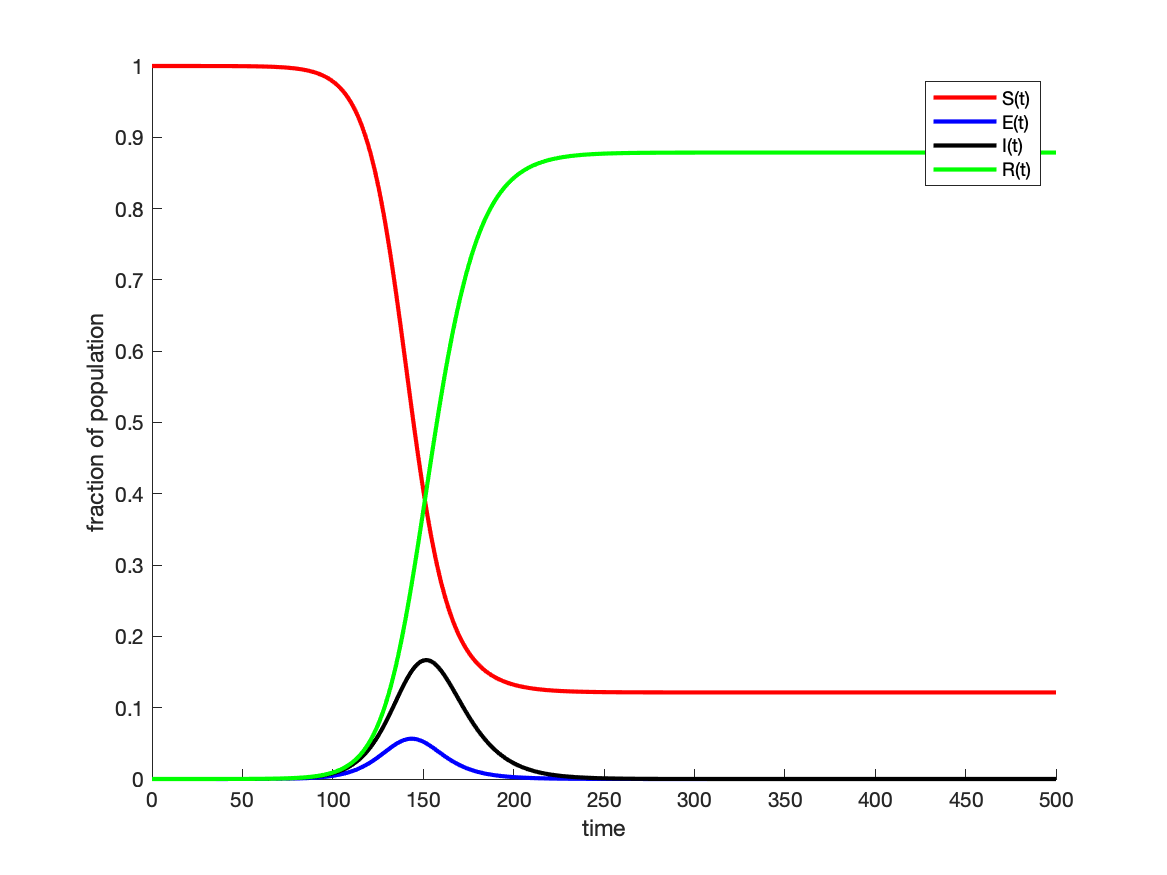
\includegraphics[scale=0.3]{img/time-SEIR-0.33.png}}
        \subfloat{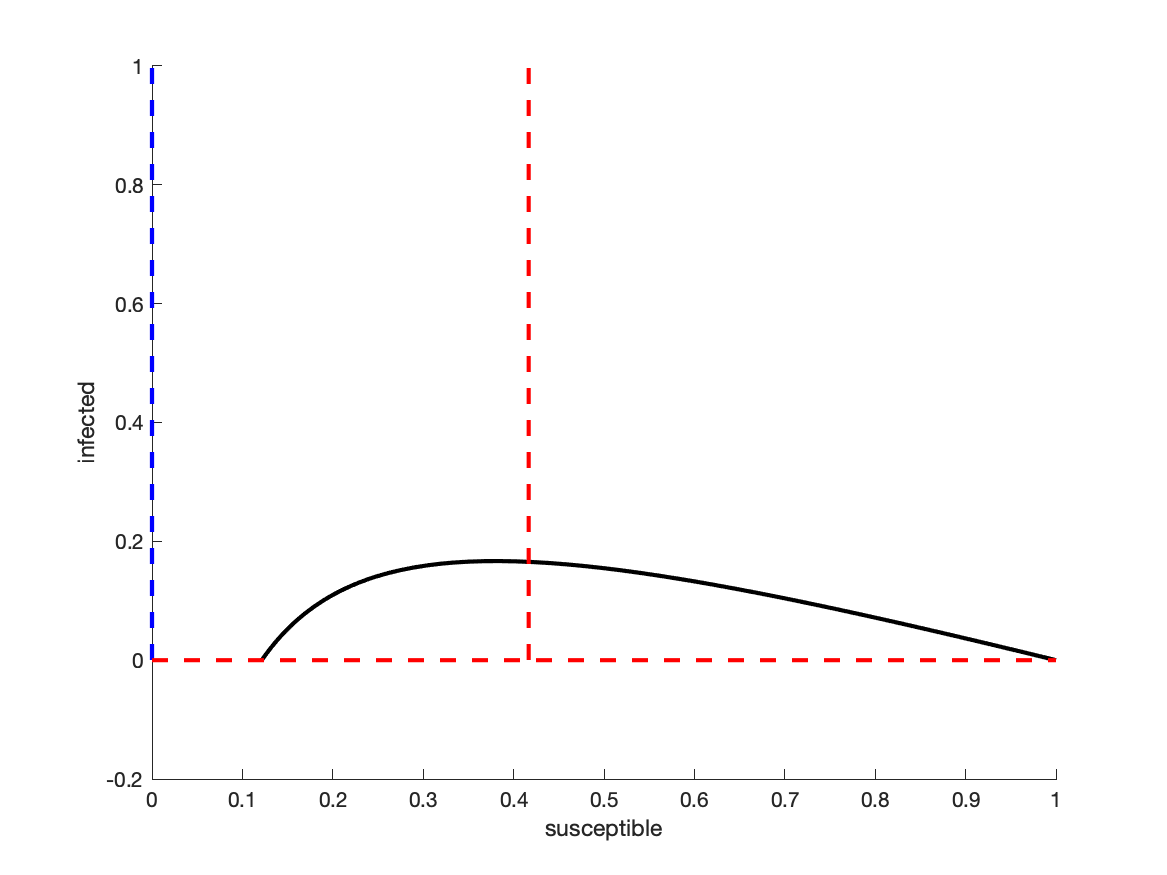
\includegraphics[scale=0.3]{img/SI-SEIR-0.33.png}}
\end{figure}
\begin{figure}[H]
        \centering
        \subfloat[$a=1$]{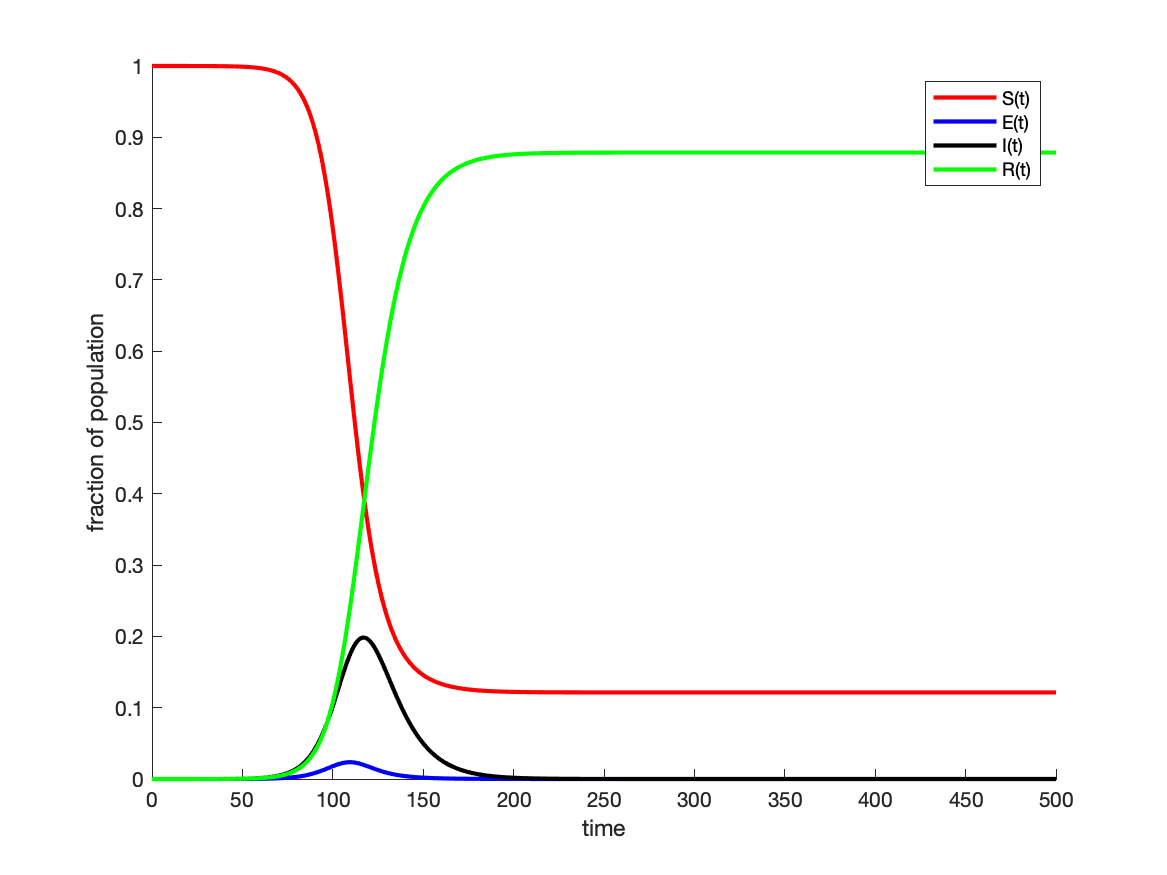
\includegraphics[scale=0.3]{img/time-SEIR-1.00.png}}
        \subfloat{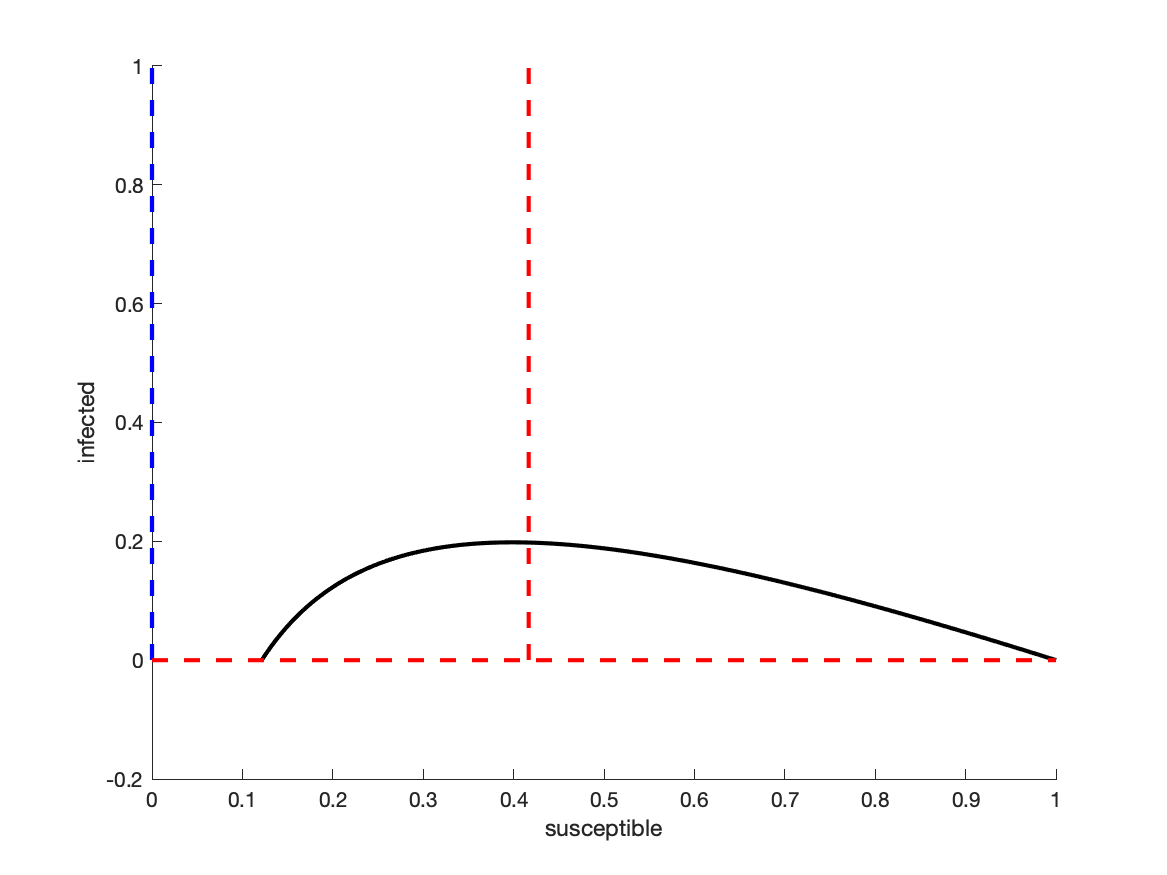
\includegraphics[scale=0.3]{img/SI-SEIR-1.00.png}}
\end{figure}
and the statistics for each are
\begin{center}
        \begin{tabular}{|c|c|c|c|}
                \hline
		$a=$ & $1/9$ & $1/3$ & $1$ \\
                \hline
		Days until peak & 235.5 & 151.3 & 117.1 \\
		Height of peak & 0.11 & 0.17 & 0.20 \\
		Final epidemic size & 0.8786 & 0.8786 & 0.8786 \\
		\hline
	\end{tabular}
\end{center}
As $a$ increases, the peak becomes earlier and more pronounced, similar to the SIR model. Increased $a$ in the SEIR model corresponds to a faster rate of movement out of the ``exposed" group and into the ``infected" group, essentially decreasing the effect that the ``exposed" group has on the projections of the model. The weaker the effect of the ``exposed" group, the closer the SEIR model's projections are to those of the SIR model. Conversely, as $a$ decreases, it takes longer to actually become infected. This results in a lower and delayed infection peak, as well as lower infection counts relative to the size of the susceptible population. One final notable point is that as $a$ changes, the final number of infected individuals does not noticeably change. An increased $a$ will ``spread out" the infection over time, but it will not affect how many people ultimately contract the disease.

%%%%%%%%%%%%%%%%%%%%
% Predicted vs. Actual Peak
%%%%%%%%%%%%%%%%%%%%

\subsection{Predicted vs. Actual Peak}

Based on the SIR model, the peak in the US would be expected to occurs around June 16. Based on the SEIR model, it would be expected around August 8. Based on actual data, a peak in US cases appears in mid-to-late July, which is in between the two expected dates but closer to the prediction of the SEIR model. One possible explanation for this difference between the model and reality is homogeneity of the US population and COVID being more complex than the SIR or SEIR models can express. Both models assume constant transmission rates, but lockdowns in the US, differing population densities, and also different susceptibilities to the disease due to genetics and age complicate this. In addition, some people who have contracted COVID have contracted it more than once, meaning that there might actually be a small flow from $R$ to $S, E,$ and $I$ that is not considered in either of our models.

%%%%%%%%%%%%%%%%%%%%
% Difference in $\rr$ Values
%%%%%%%%%%%%%%%%%%%%

\subsection{Difference in $\rr$ Values}

One potential reason for the difference in $\rr$ predictions between the SIR and SEIR models is the difference in expected infection counts between the models. As noted earlier, the SIR model predicted earlier, larger peaks, while the SEIR model predicted later, lower peaks. Since the actual peak of the disease in the US seems to have occurred before the SEIR-predicted peak, the data has to at some point grow faster than what was predicted by the model. Then, it appears to the model that the $\rr$ value is higher than the first 20 days of data suggested.

Conversely for the SIR model (whose predicted peak was before the actual peak in the US), the observed cases had to at some point grow slower than predicted by the SIR model. In this case, it would appear to the model that the true value of $\rr$ is lower than the first 20 days of data suggested.

Based on these two observations, it seems reasonable that the $\rr$ values predicted by the SIR model were consistently less than those predicted by the SEIR model.

\section{Data Exercise}

The cumulative cases per country (with timelines normalized by starting at $t=0$ when a country reaches 2 million cumulative cases per million), as well as the logarithm of the cumulative cases, are plotted below.
\begin{figure}[H]
        \centering
        \subfloat[$a=1$]{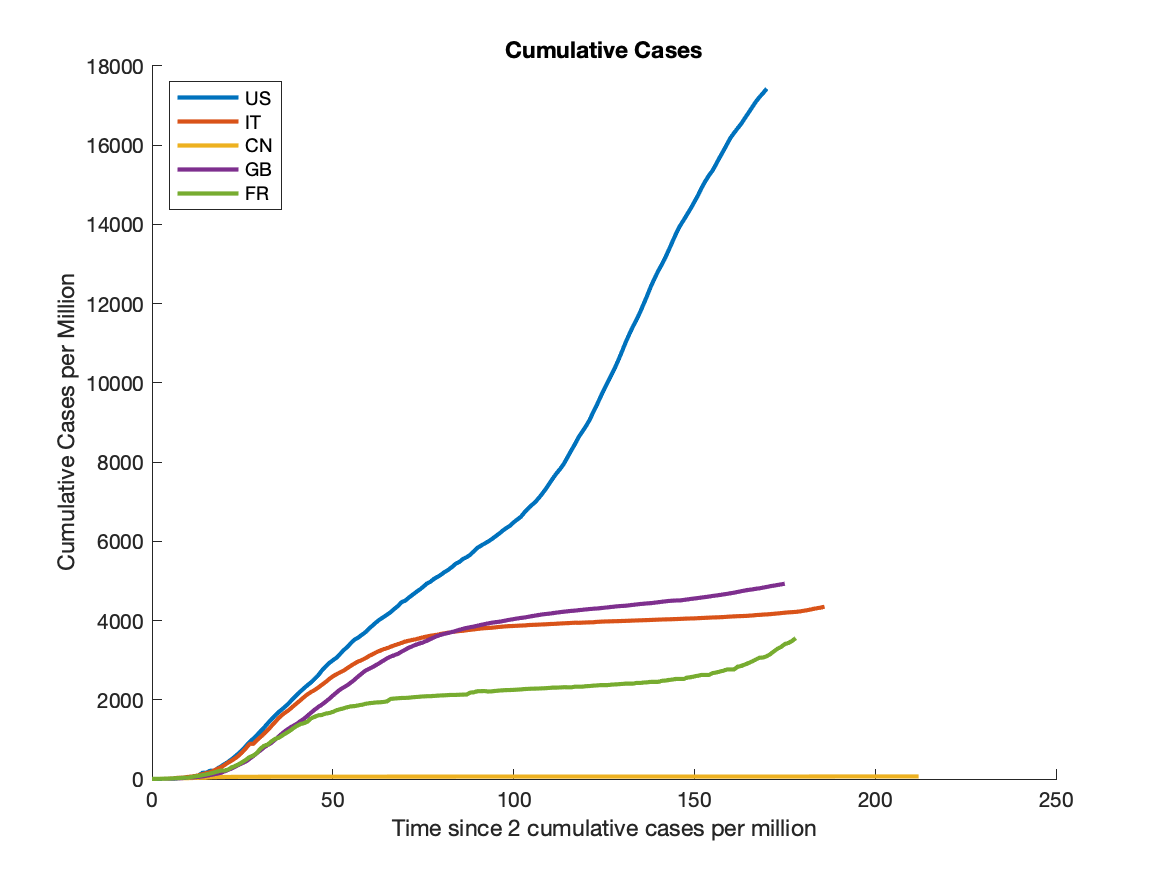
\includegraphics[scale=0.4]{img/cum-cases.png}}
        \subfloat{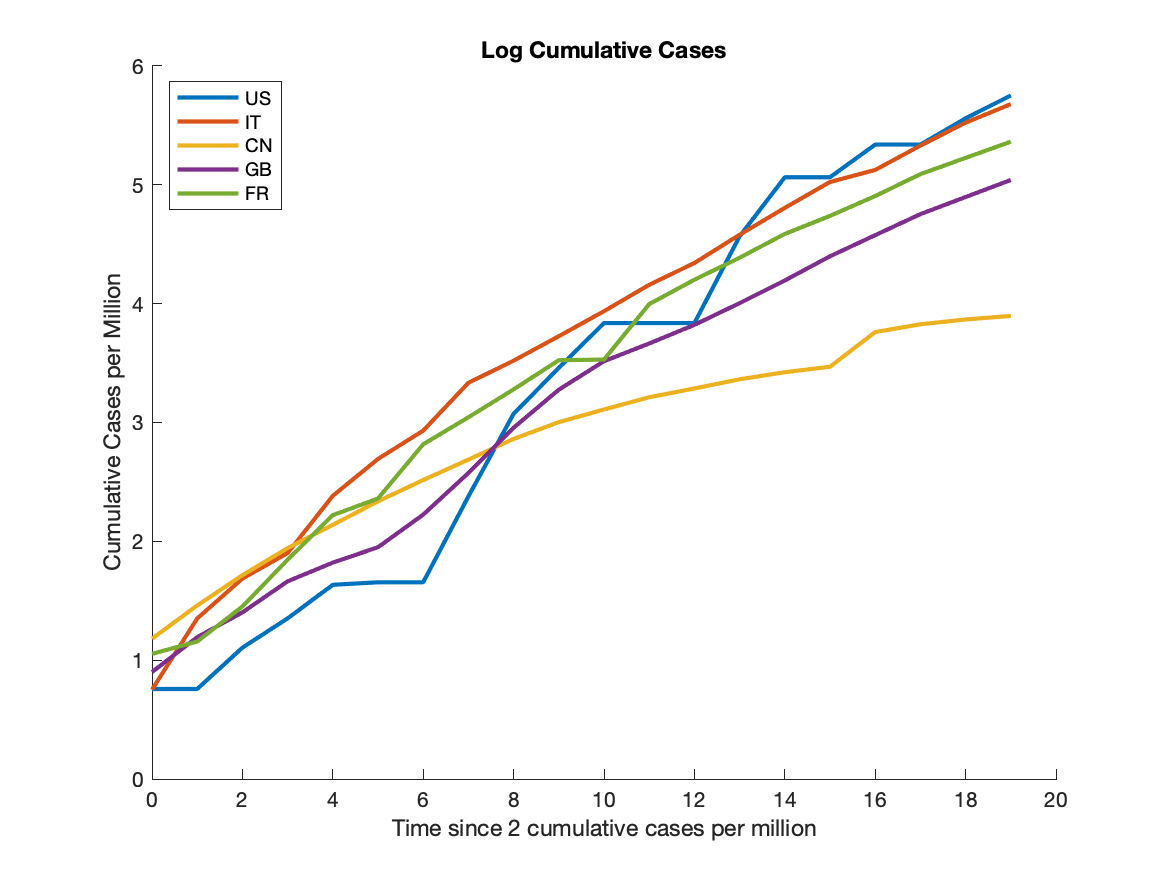
\includegraphics[scale=0.4]{img/log-cum-cases.png}}
\end{figure}
The doubling time $T_d$ for a country was computed by first fitting a linear line through that country's logarithmic cumulative cases from the first 20 days after $t=0$. The $\alpha$ parameter was set to the slope of this linear fit, and the doubling time was approximated by $T_d = \ln(2)/\alpha$. The $\alpha$ and $T_d$ estimates are reported below.
\begin{center}
        \begin{tabular}{|c|c|c|}
                \hline
		& $\alpha$ & $T_d$ \\
                \hline
		US & 0.294 & 2.360 \\
		Italy & 0.247 & 2.811 \\
		China & 0.137 & 5.057 \\
		Great Britain & 0.225 & 3.079 \\
		France & 0.235 & 2.954 \\
                \hline
        \end{tabular}
\end{center}
Since $I_0 = 2$ for each country, we expect to hit 5 million cases when $t$ satisfies
\begin{align*}
	5 &= 2 e^{\alpha t} \\
	t &= \frac{\ln (5/2)}{\alpha} \\
	t &= \frac{\ln 5}{\alpha} - T_d
\end{align*}
Based on this, the expected vs actual time for each country reaching 5 million cases is reported below.
\begin{center}
        \begin{tabular}{|c|c|c|}
                \hline
		\multicolumn{3}{|c|}{Days until 5 million cases} \\
		\hline
		& Predicted & Actual \\
		\hline
		US & 3.12 & 5 \\
                Italy & 3.72 & 3 \\
                China & 6.68 & 3 \\
                Great Britain & 4.07 & 4 \\
                France & 3.90 & 4 \\
                \hline
        \end{tabular}
\end{center}
The predictions seem to match up with reality to some extent, although there are some deviations. Great Britain and France are both very close to their predictions, although the prediction for the US is too high and the predictions for China and Great Britain are too low.

In general, the predicted time is too high (except in the case of the US). A number of factors could have influced this error. There is general error stemming from stochasticity of populations and possibly incorrect data points. For Italy and China, the possibility of delayed reporting could also have made the estimates too high. If a large number of cases went unreported, then the disease would have larger growth than accounted for by the model, resulting in predictions that overestimate how long it will take for the disease to spread. This seems reasonable for China, as the virus originated there, giving the government little time to prepare testing resources. This also makes sense for Italy, which received much negative press for being seemingly overrun by the virus. If a country's healthcare system is operating at full capacity, inexhaustive testing would be a natural effect.

For the United States, preemptive warning from witnessing other nations dealing with the disease might have allowed for precautions to be taken to slow down the spread of the virus. The population of the US is also heterogeneously spread throughout the country, and some initial infection hotspots (like in Washington state) could have been in less densely population regions of the country, resulting in slower spread.

\end{document}
